\section{Objetivos y contextualización}

  Actualmente, la empresa tiene más de 700 clientes activos, cada uno con diferentes contratos, o condiciones comerciales, y se utiliza un archivo de Excel para mantener estas condiciones actualizadas. Al mismo tiempo, este Excel también contiene la forma en que se calculan los costos totales por el uso del servicio para cada cliente. Similar a lo que ocurría con la falta de pruebas automatizadas, también resulta curioso el hecho de que Beetrack, siendo una empresa SaaS y teniendo su propio ERP, utilice esta plantilla para calcular cuánto cobrarle a los clientes. Es por lo anterior que decidió crear un servicio especializado en el almacenamiento y cálculo de estas condiciones comerciales, cuyo único propósito fuese resolver el problema de cómo calcular los costos por cliente y poder almacenar los modelos que representaran los contratos generados con estos.
  
  Uno de los puntos más cruciales sobre este servicio y su contexto es el hecho de que ya se había intentado dos veces algo similar. El primer intento fue mediante un desarrollo interno en el ERP, que resultó no tener el rendimiento esperado en términos de precisión al momento de facturar y se concluyó que no era responsabilidad de \textit{Hive} como tal tener esta información. El segundo intento fue la migración de estos planes a un proyecto que, en su minuto, se encontraba en fase \textit{beta} en Hubspot, en el cual se prometía poder tener la información siempre actualizada. Finalmente terminó ocurriendo lo mismo que en el primer intento, pero con mejor precisión al momento de facturar de manera automática, entregando, en el mejor de los casos, una precisión de 43\%.

  Teniendo en consideración los requisitos y los resultados anteriores, los objetivos principales del proyecto fueron dos. El primero fue construir un modelo lo suficientemente flexible como para poder abarcar los diferentes tipos de ventas que los vendedores realizan, tanto para productos como servicios. El segundo objetivo fue el programar un servicio de resolución comercial, o calculadora, que fuese, nuevamente, lo suficientemente flexible como para poder abarcar el modelo, pero que al mismo tiempo no necesitara información contextual más allá del uso para saber cuánto cobrarle a cada cliente, mientras que al mismo tiempo entregue glosas prehechas por producto.

  El equipo de operaciones decidió no acoplar este proyecto a \textit{Hive} de manera de evitar el cruce indebido de información, poder mantener las ideas aisladas y comenzar distribuir los servicos que posee el ERP. Lo anterior sumado al hecho de que se prevee que, eventualmente, otros servicios y productos de la empresa, tales como el \textit{Customer Portal}, consuman los recursos expuestos por este servicio de manera de que los clientes también puedan saber cuánto se les cobrará o el nivel de costo que tienen para un día determinado del mes. Como se puede ver en la figura \ref{fig:arquitectura}, del capítulo \ref{metodologias}, la arquitectura que se decidió utilizar es una en la cual el servicio de condiciones está aislada del ERP, mientras que al mismo tiempo no limita a que otro servicio pueda consumir la información del servicio nuevo, lo cual hubiese ocurrido en caso de haber escrito el código en \textit{Hive} dada su naturaleza monolítica.

\section{Desarrollo}

  \subsection{Modelamiento}
    \label{modelamiento}

    El proceso de desarrollo del nuevo servicio de condiciones comerciales comenzó con un análisis de los diferentes planes existentes y que se encontraban en uso por parte de la empresa. Luego de realizar este análisis se definieron 4 modelos diferentes a nivel de bases de datos que permitirían almacenar de manera flexible las condiciones con las cuales se les factura a los clientes. 
    
    En primer lugar se tiene el modelo del plan, en este se almacena la condición comercial como tal, junto con una descripción del uso que puede tener esta condición y el producto y moneda asociado a la condición. Dentro del campo ``\texttt{condition}'' se almacena el tipo de tramo y costos asociado que tendrá por ellos. Se decidió que se puede tener tres tipos de tramos diferentes: base, variable y por paso.
    
    A continuación se detalla cada tipo de tramo:
    \begin{enumerate}
      \item Tramo base: va desde cero unidades hasta la cantidad de unidades determinada con un costo fijo total por esas unidades. Solamente se puede tener un tramo de este tipo por plan.
      \item Tramo variable: funcionan mediante una definición de inicio a final del tramo en término de cantidad de unidades, con un precio unitario por la cantidad de unidades utilizadas. Se pueden tener entre cero e infinitos tramos variables por plan.
      \item Tramo por pasos: se utiliza para poder representar los productos que se venden mediante paquetes; esto es especialmente útil para el servicio de correos en el cual se cobra mediante paquetes de 10.000 correos, siendo los primeros 10.000 gratis y los siguientes teniendo un costo de 1 UF por bolsa adicional. Este tipo de tramo es excluyente con los dos anteriores y funciona de manera recurrente.
    \end{enumerate}
    
    Adicionalmente, el campo ``\texttt{condition}'' contiene dos variables utilizadas al momento de calcular el costo total de la factura de un cliente. Estos se detallan a continuación:
    \begin{enumerate}
      \item \texttt{general\_minimum}: se utiliza para asegurar un monto mínimo de facturación del producto independiente del uso del cliente. Se pone en uso una vez que ya se haya calculado el costo por el uso que el cliente haya tenido.
      \item \texttt{add\_base\_to\_variable}: se utiliza al momento de calcular el costo del uso del producto y sirve para saber si el plan que se negoció con el cliente se cobra sumando el costo base o utilizando el costo unitario del tramo variable en caso de aplicar.
    \end{enumerate}
    
    El esquema de información del campo ``\texttt{condition}'' se puede ver en la figura \ref{fig:cc_condition_schema}, mientras que en la figura \ref{fig:cc_pricing_chart} se puede observar una manera visual de entender el modelo de precios y condiciones comerciales de los clientes. Es importante mencionar que se hizo un uso avanzado de RoR mediante la creación de artefactos de validación que permiten mantener los esquemas de datos establecidos en la figura \ref{fig:cc_condition_schema}. Al mismo tiempo, también se utilizó validación de los datos en si mismos, forzando a que siempre se tengan tramos positivos, sin sobrelape y que sean rangos acotados, de manera de que las condiciones siempre tengan las formas de la figura \ref{fig:cc_pricing_chart}.
    
    \begin{figure}
      \centering
      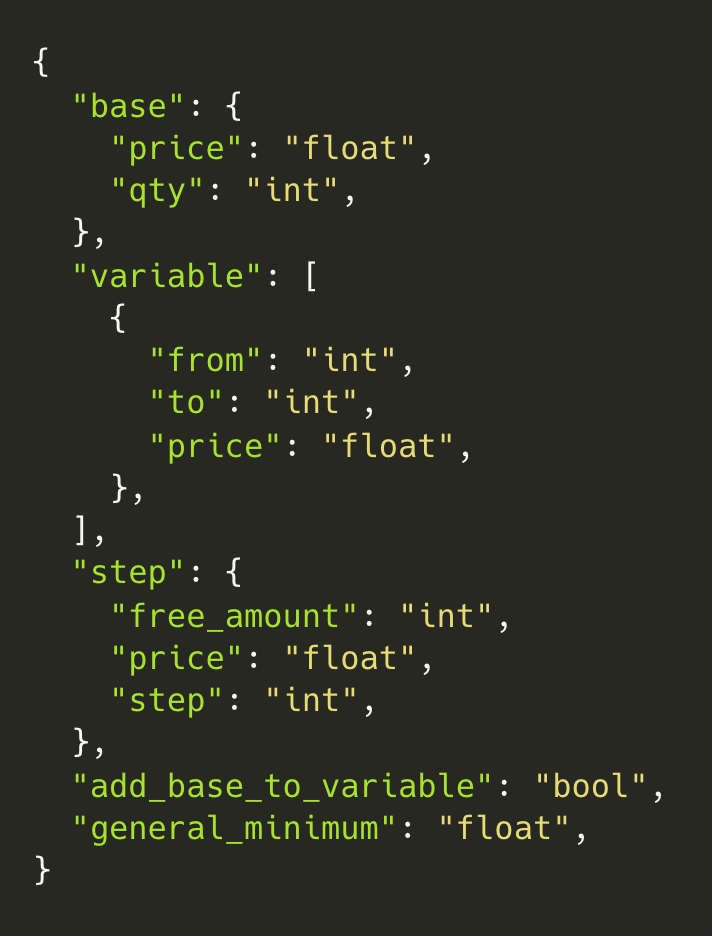
\includegraphics[width=0.4\linewidth]{figures/cc/cc_condition_schema.png}
      \caption{Esquema de información de condición comercial.}
      \label{fig:cc_condition_schema}
    \end{figure}

    \begin{figure}
      \centering
      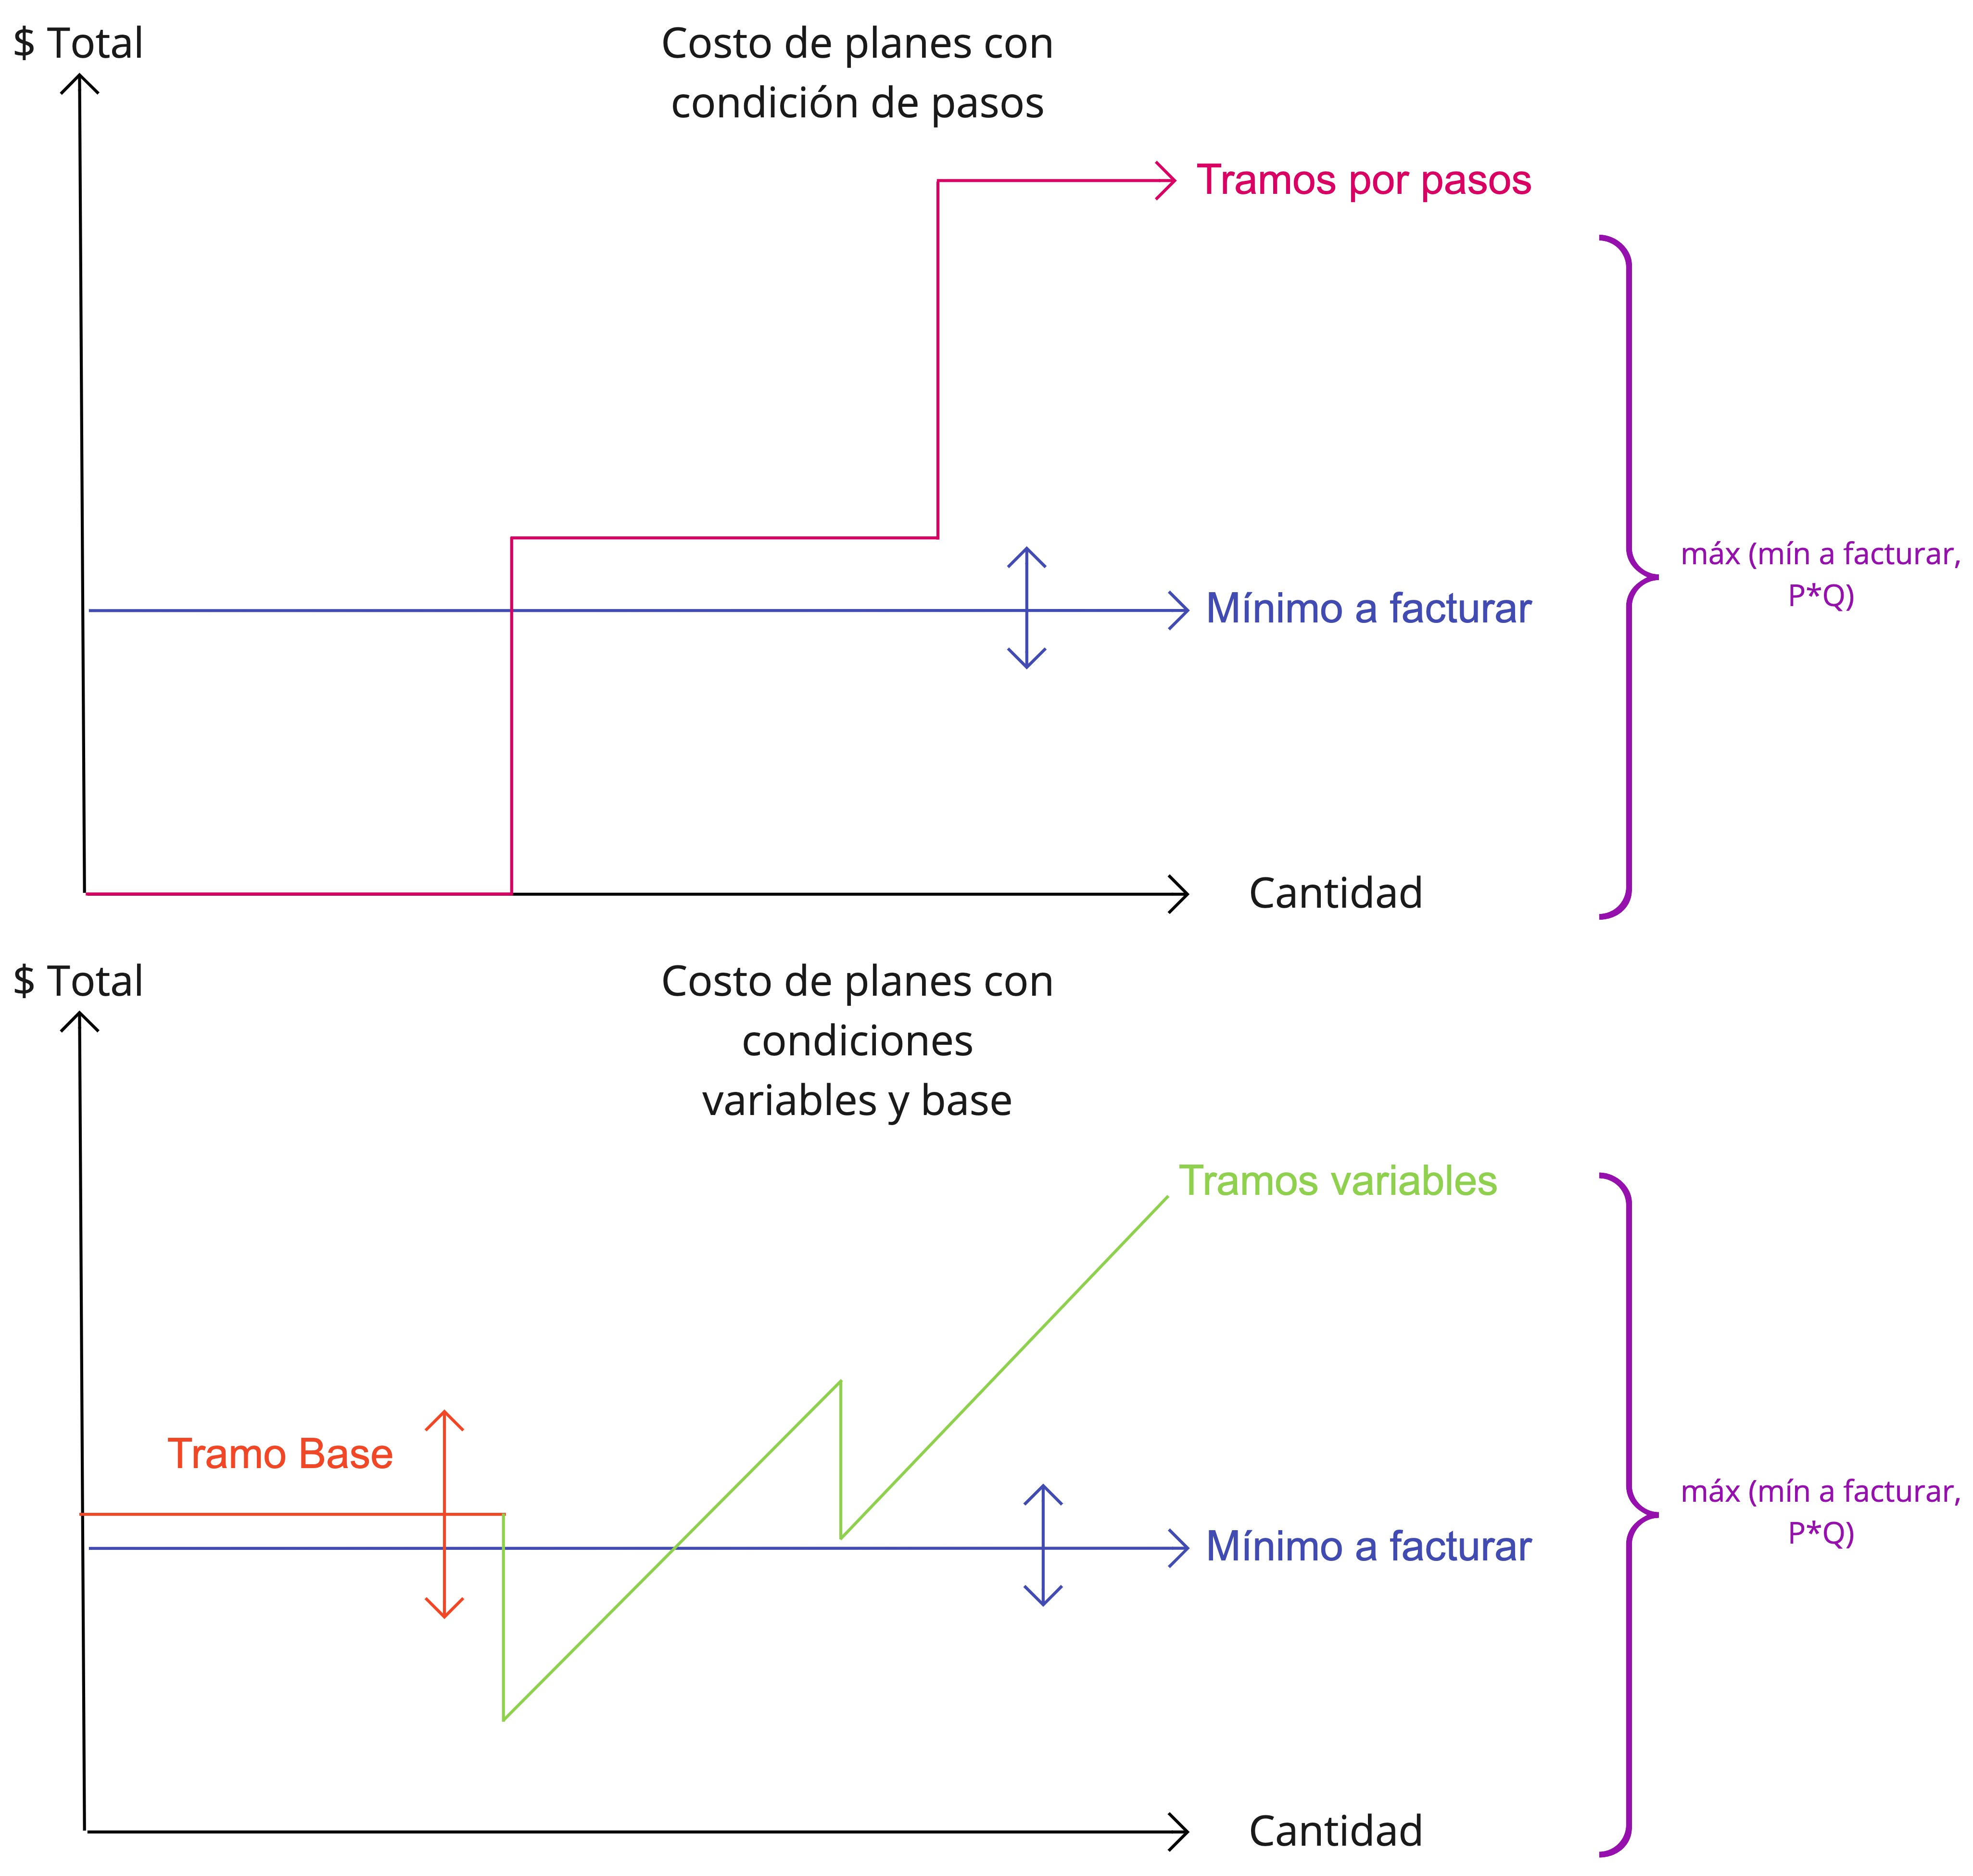
\includegraphics[width=0.6\linewidth]{figures/cc/cc_pricing_chart.jpg}
      \caption{Modelos de cobros y condiciones comerciales.}
      \label{fig:cc_pricing_chart}
    \end{figure}

    En segundo lugar, el modelo de relación plan (\texttt{plan\_relations}) tiene el rol de asociar el contrato del cliente con el plan creado de manera desacoplada y permitiendo la reutilización de planes estándares. 
    
    En tercer lugar, ``\texttt{plan\_relation\_proposals}'' tiene el propósito de permitir que se pueda tener una agrupación de relaciones de planes en un mismo modelo en caso de que un vendedor haya pactado con un cliente condiciones no estándar. Las condiciones estándar se definieron en conjunto con los vendedores a lo largo de múltiples reuniones y una posterior validación de Felipe Porter, jefe del área de ventas de la empresa. En caso que las condiciones que un vendedor otorgó no sean las predefinidas se acordó que estas requerirían aprobación de Felipe Porter o Sebastián Ojeda (CEO). En caso contrario, las condiciones para el cliente determinado se aprueban de manera automática y se pueden utilizar al momento de facturar.
    
    En cuarto, y último lugar, el modelo ``\texttt{comments}'', tiene el propósito de contener el cuerpo del comentario por parte del vendedor en caso de que quiera hacer notar algo de los planes que está creando.

    En la figura \ref{fig:cc_relations} se puede observar los diferentes modelos y sus relaciones, junto con sus campos y tipos de datos por campo.
    
    \begin{figure}
      \centering
      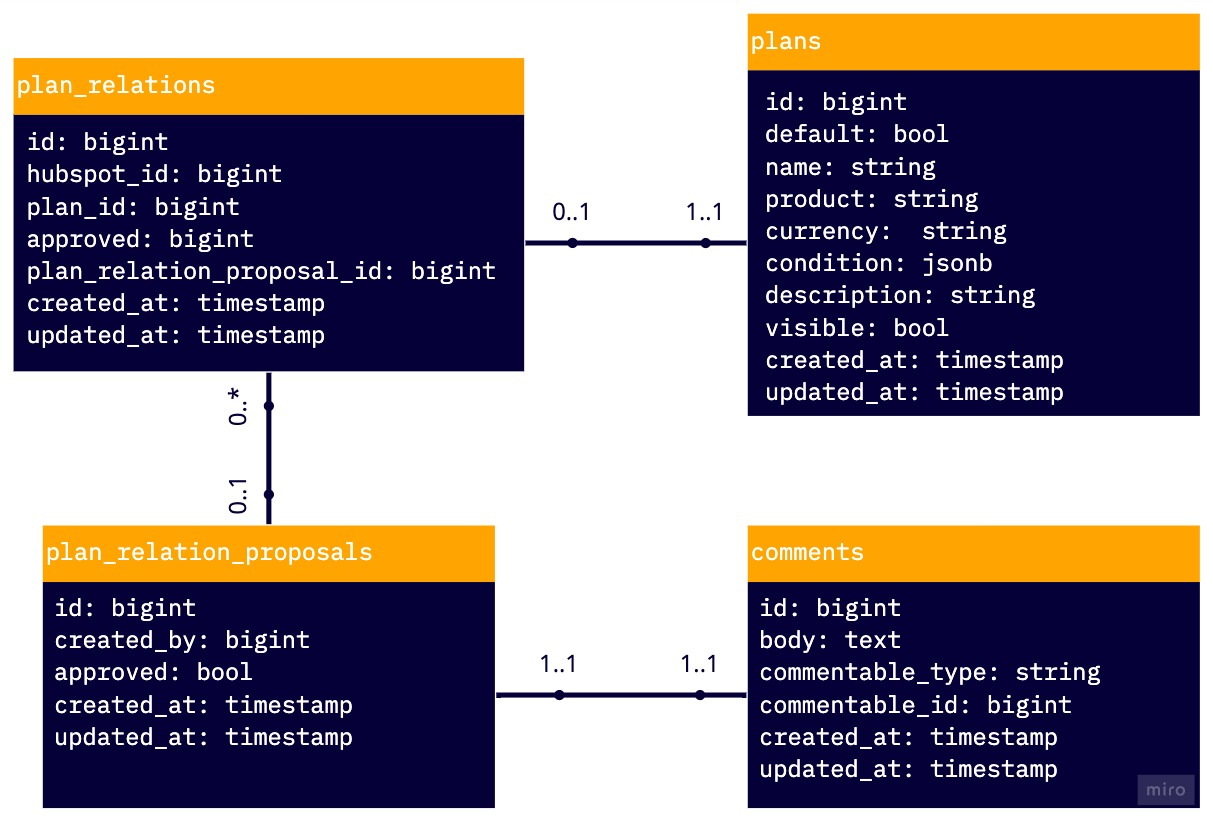
\includegraphics[width=0.75\linewidth]{figures/cc/cc_relations.jpg}
      \caption{Relaciones de modelos de condiciones comerciales.}
      \label{fig:cc_relations}
    \end{figure}

  \subsection{\textit{Solver} de condiciones y arquitectura}
    \label{solver_y_arquitectura}

    El paso siguiente a la creación de los modelos a utilizar, fue el de la generación de un módulo dentro del servicio de condiciones comerciales  que permitiese calcular la facturación adecuada para un cliente en específico dado el uso que este tuvo durante el mes. El módulo de cálculo se basa en un servicio específico para cada producto existente dentro de la empresa, es decir, por cada producto se tiene un servicio específico para calcular y resolver el cobro a realizar para ese producto dado el uso entregado.

    La información externa que el servicio de cálculo requiere es el identificador del cliente, junto con el uso de los productos. El servicio de cálculo, con la información entregada, se programó de manera de que pase por una calculadora general y delegador; de este modo se subdelega el cálculo del monto a facturar a los subservicios específicos por productos. Este último diseño se basó en la implementación del patrón de diseño ``mediador'', en el cual se restringe las comunicaciones directas entre los objetos, forzándolos a colaborar únicamente a través de un objeto mediador \cite{pattern_mediator} y ``fachada'', en el cual se proporciona una interfaz simplificada a una biblioteca \cite{pattern_facade}. Por otro lado, la información del tipo de cobro se obtiene directamente desde la base de datos del servicio mediante el producto que se quiere calcular y el identificador del cliente para el cual se está calculando.
    
    Una vez que se realiza el cálculo por producto, el servicio retorna la información a un método que agrupa los diferentes resultados, suma el total y entrega un desglose por producto y por moneda, especificando el servicio de resolución utilizado, junto con la glosa a utilizar al momento de generar la factura en el ERP. En la figura \ref{fig:cc_calculator} se puede ver de manera general el flujo utilizado en el \textit{solver} y calculadora de costos.

    \begin{figure}
      \centering
      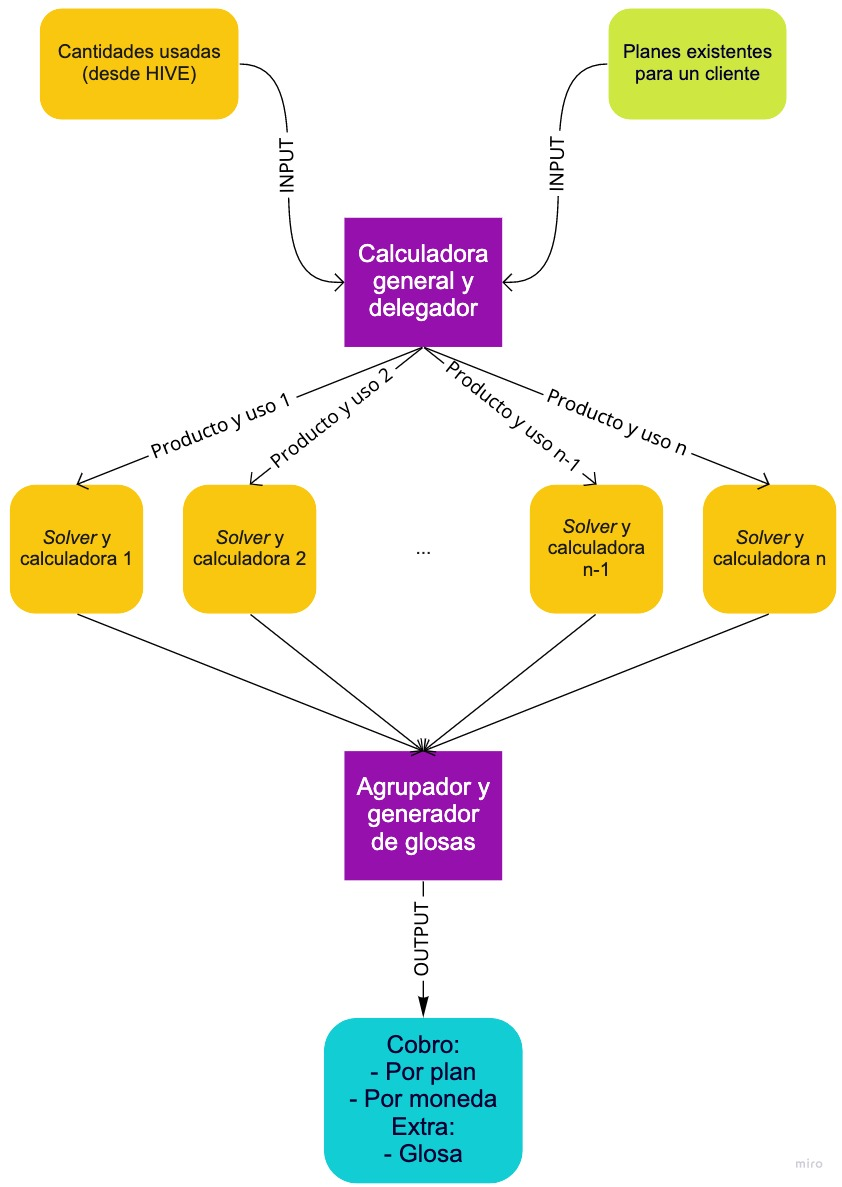
\includegraphics[width=0.5\linewidth]{figures/cc/cc_calculator.jpg}
      \caption{Esquema de delegación de \textit{solver} y calculadora.}
      \label{fig:cc_calculator}
    \end{figure}


    Posteriormente, una vez que el alumno terminó de programar el servicio de cálculo, este procedió a conectar el ERP con el servicio de condiciones comerciales. Para realizar la conexión se optó por utilizar una API con GraphQL expuesta por parte del servicio de condiciones comerciales. Por parte de \textit{Hive}, se utilizó Artemis, una librería de RoR que permite conectar el cliente, en este caso el ERP, con la API de manera casi invisible, exponiendo los métodos como si fuesen nativos de la aplicación \cite{artemis_gem}. Esta implementación permite, al mismo tiempo, que otras aplicaciones dentro de Beetrack consuman el servicio mediante el ERP, en caso de ser requerido. En la figura \ref{fig:cc_arquitectura} se puede observar la arquitectura con los dos \textit{pods} diferentes de GKE, uno para el ERP y otro para el servicio de condiciones comerciales y su comunicación mediante una API con GraphQL.

    \begin{figure}
      \centering
      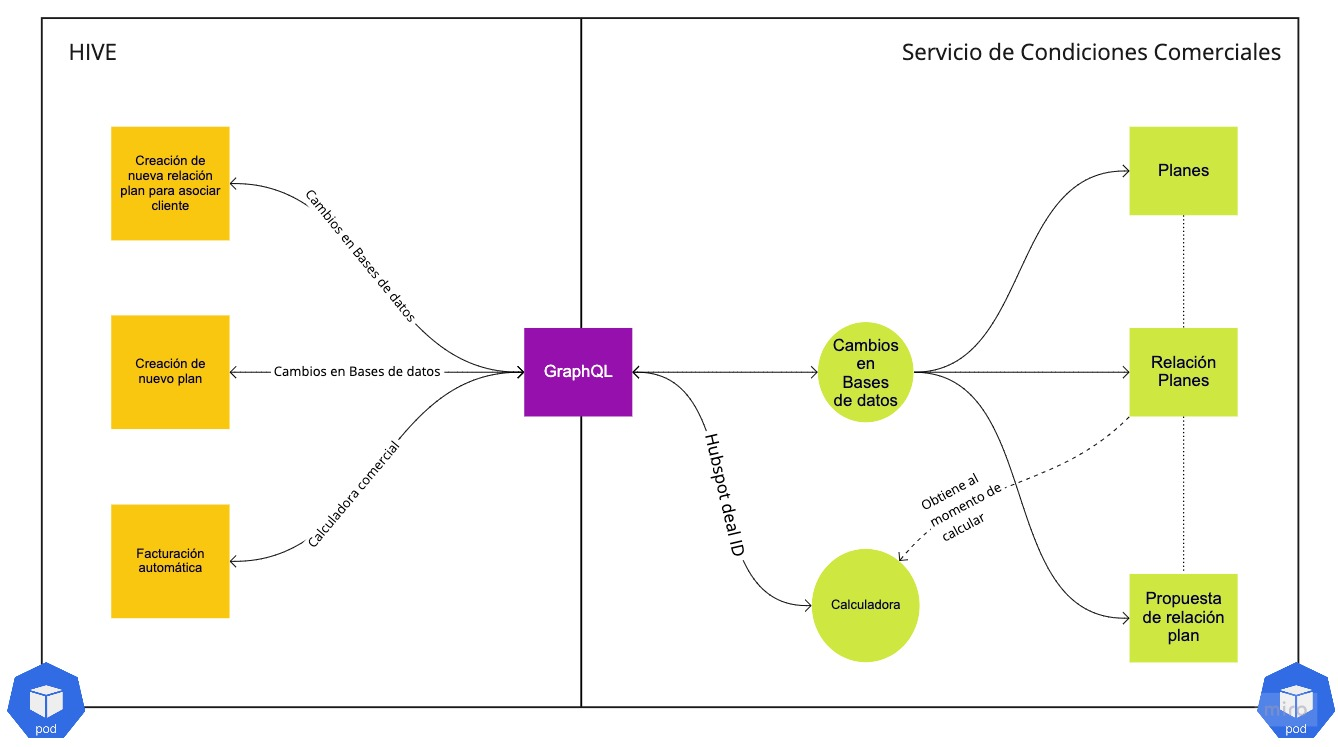
\includegraphics[width=\linewidth]{figures/cc/cc_arquitectura.jpg}
      \caption{Relaciones de modelos de condiciones comerciales.}
      \label{fig:cc_arquitectura}
    \end{figure}
    
  \subsection{\textit{Refactoring} y generación de facturas automáticas}

    Una vez que el alumno conectó el servicio de condiciones comerciales al ERP, este procedió a desacoplar el sistema antiguo que generaba las facturas de manera automática los 28 de cada mes. Esto se hizo en favor del servicio nuevo externo a \textit{Hive}, adaptando el código antiguo al sistema nuevo. Esto permitió un desacoplamiento de la lógica por parte del ERP, delegándosela al sistema creado. Por otro lado, el cambio implicó la eliminación de más de mil líneas de código en el ERP, con la generación de glosas y cálculo de montos a facturar siendo los princiaples elementos removidos.

    Posteriormente, el alumno le pidió al CEO de la empresa, Sebastián Ojeda, el archivo de Excel en el cual mantenía las condiciones comerciales de manera de poder poblar el servicio. Para esto, el estudiante se comprometió a no entregar los datos de facturación a nadie sin autorización previa, manteniendo un código ético intachable dada la sensibilidad de la información. Adicionalmente, dado el elevado número de contratos de la empresa (mayor a 700), se decidió escribir código que transcribiese el archivo excel al formato del servicio, generando más de 1500 planes diferentes válidos.

    Luego de que se transcribieran los planes generados al servicio de condiciones comerciales, el universitario se coordinó con el equipo de \textit{Data Science} de manera de poder hacer simulaciones de facturación antes de poner en funcionamiento el servicio de generación de pre-facturas reales. De esta manera, se simuló una ejecución del problema real y se puso a prueba el código desarrollado para tener conocimiento de cuán preciso era. El alumno trabajó con el equipo de \textit{Data Science}, dado que este es el encargado de la carga de datos de uso de los clientes, por lo que se pudo generar simulaciones con diferentes niveles de uso y para diferentes clientes. Los resultados obtenidos fueron altamente prometedores, resultando en una precisión de facturación de 87,9\%. Finalmente, el 28 de octubre corrió el servicio de generación automática de pre-facturas exitosamente y recibió comentarios muy positivos por el equipo contable de la empresa dado que tuvieron que modificar muy pocas pre-facturas antes de emitirlas.

  \subsection{Creación de condiciones por parte de vendedores y aprobación de gerentes}
    En paralelo, junto con la generación automática de pre-facturas, el alumno trabajó en 4 vistas dentro del ERP, las cuales corresponden a dos formularios y dos vistas generales. Adicionalmente se crearon 3 plantillas de correos mediante HTML, CSS y Ruby embebido; estas se detallarán más adelante. Estas vistas fueron validadas y diseñadas junto a Grace Lillo, del equipo de \textit{design ops}, de manera de que fueran realmentes útiles para los usuarios finales. Cabe mencionar que estas vistas fueron programadas utilizando los componentes de \textit{Honeypot} en React. 
    
    % vista general de condiciones comerciales
    En primer lugar, el estudiante generó una vista general en donde los vendedores pueden ver las condiciones comerciales preaprobadas por los gerentes, de manera de poder tener una noción de cuáles son las condiciones de cada plan antes de utilizarlas para un cliente determinado. A continuación, en la figura \ref{fig:cc_visible}, se puede ver la vista mencionada anteriormente.

    \begin{figure}[H]
      \centering
      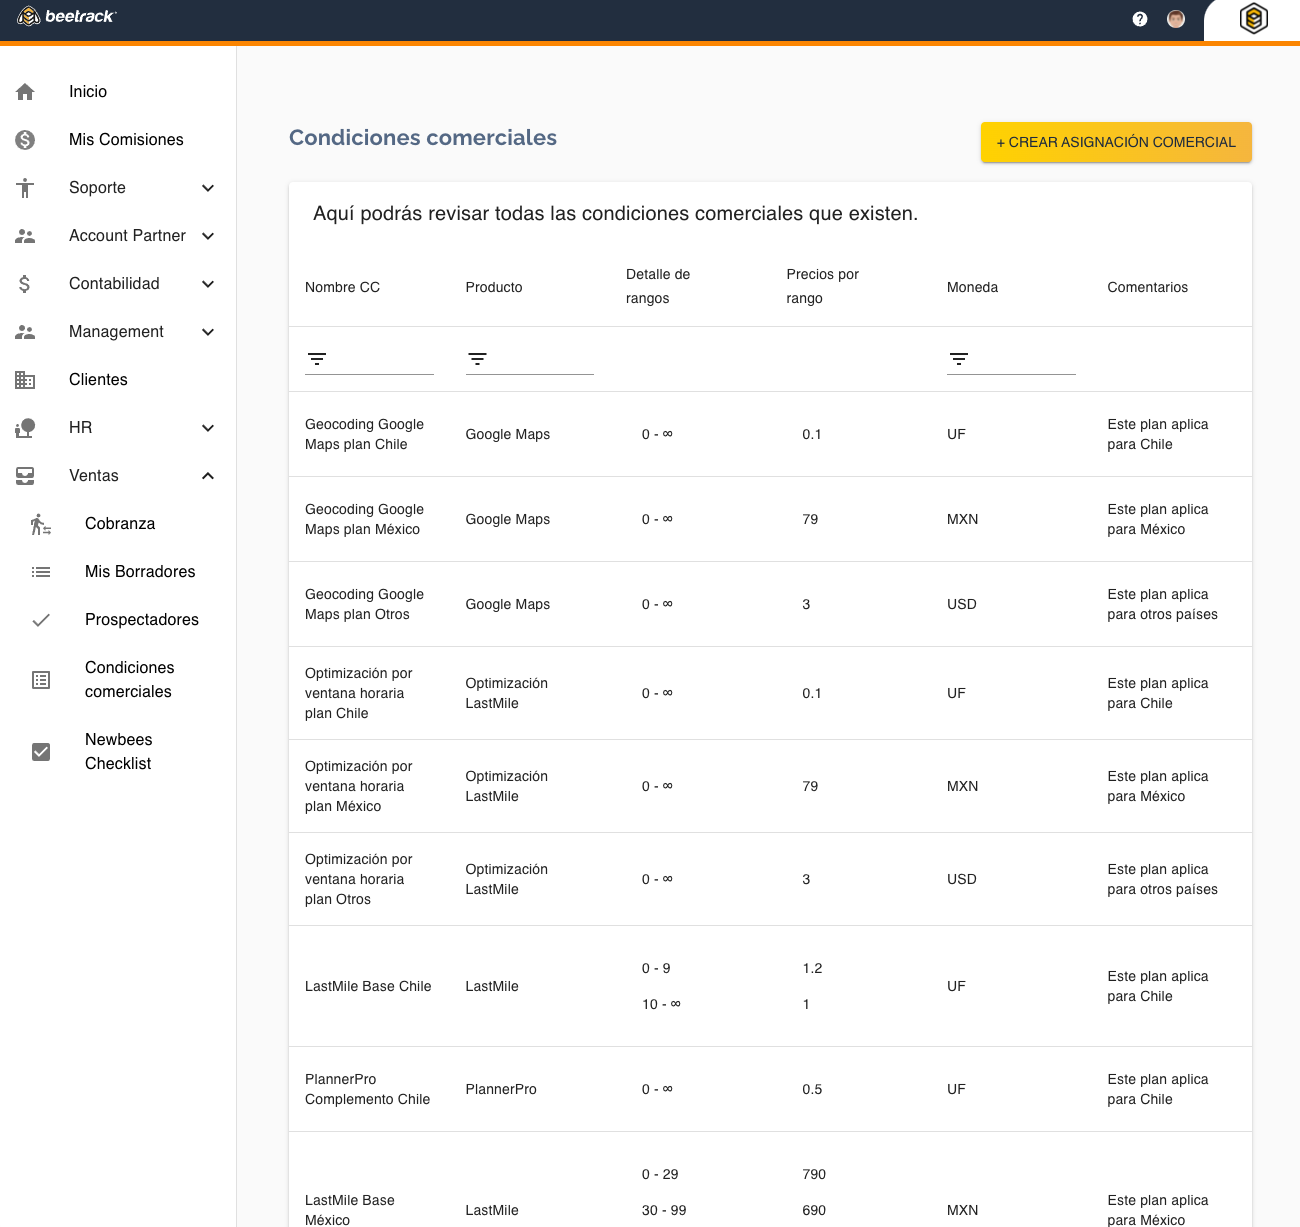
\includegraphics[width=0.6\linewidth]{figures/cc/vistas/cc_visible.png}
      \caption{Vista general de condiciones comerciales preaprobadas.}
      \label{fig:cc_visible}
    \end{figure}

    % vista de creacion de condicion comercial nueva por vendedor
    En segundo lugar, el alumno realizó una formulario que le permite a los vendedores crear asociaciones comerciales, es decir, asociar una condición comercial existente y preaprobada a un cliente determinado. Parte crucial del formulario es el hecho de que se puedan definir precios personalizados y montos mínimos a facturar solamente para los productos y no para los servicios, ya que esto va en línea con el plan de la empresa de tener planes estandarizados y asimilarse más a un SaaS tradicional. 
    
    Un punto importante de este flujo es el hecho de que si el vendedor cambia el precio predefinido del tramo de un producto, se notificará mediante un correo como el de la figura \ref{fig:cc_mail_new} a los gerentes de esta propuesta, de manera de que ésta pueda ser aprobada o rechazada. En caso de que el plan preaprobado no tenga cambios en los precios, este se aprobará de manera automática. Lo anterior fue un pedido específico de parte de los gerentes con el propósito de poder tener mayor control sobre los tipos de planes que crean los vendedores para así evitar la generación de esquemas poco comunes. El formulario mencionado se puede ver en la figura \ref{fig:cc_new_sales_man}.

    % vistas de nueva condicion comercial y mail
    \begin{figure}[H]
      \centering
      
\includegraphics[width=0.6\linewidth]{figures/cc/mails/cc_mail_new.png}
      \caption{Correo electrónico de solicitud de aprobación de asociación comercial.}
      \label{fig:cc_mail_new}
    \end{figure}

    \begin{figure}[H]
      \centering
      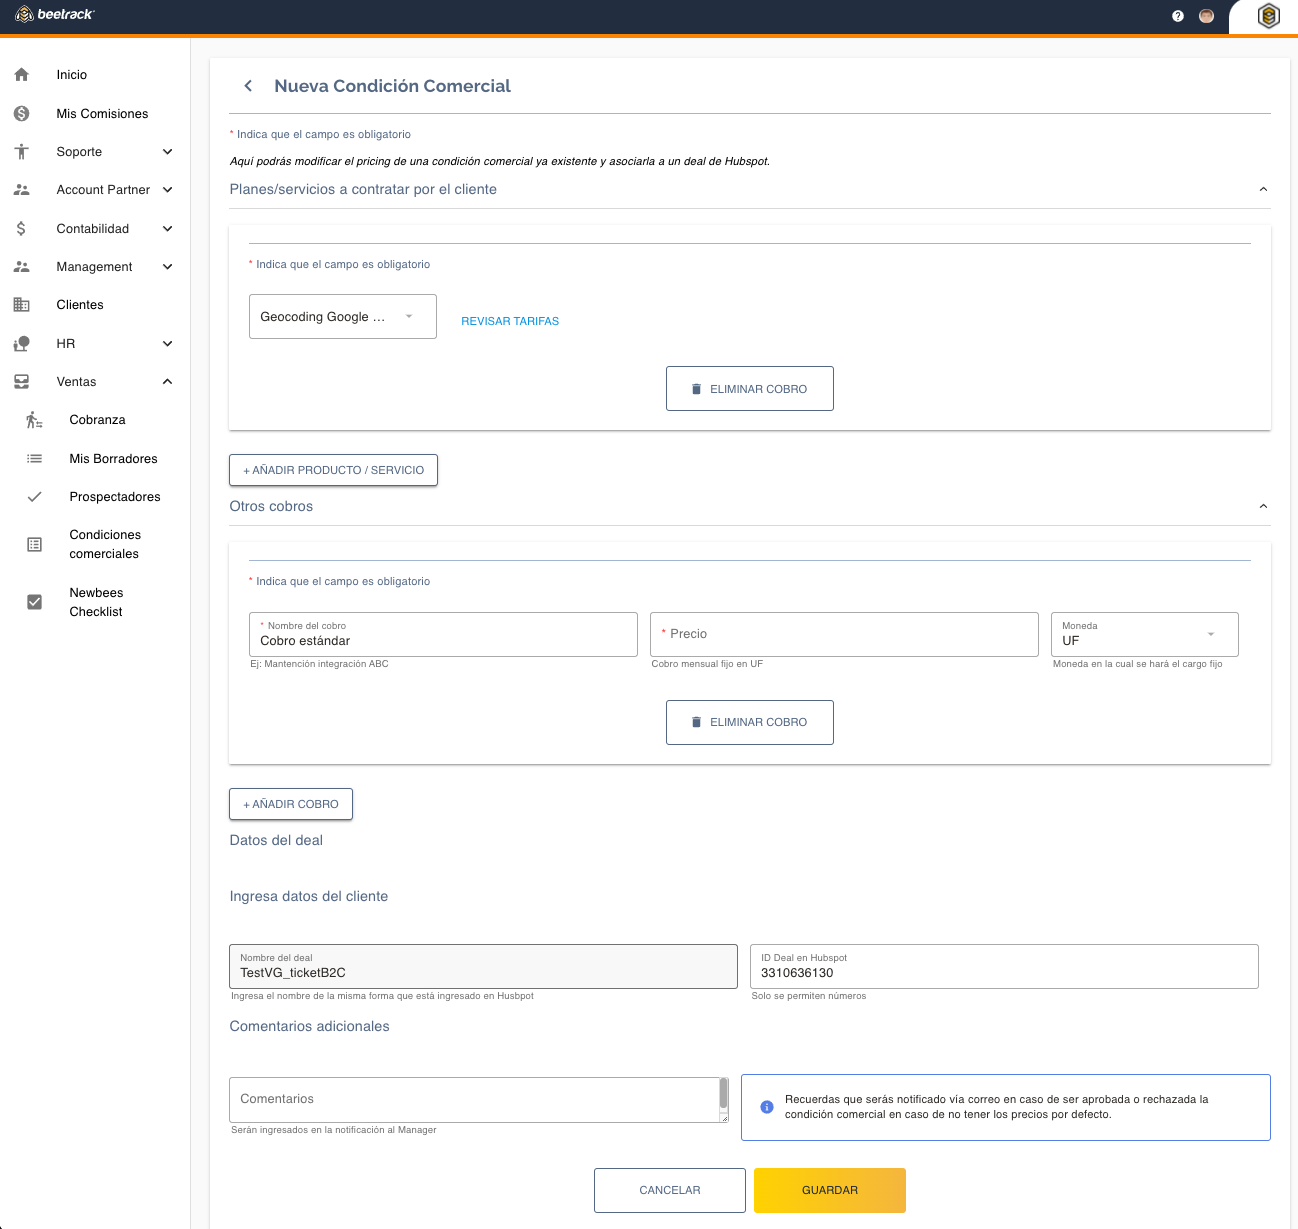
\includegraphics[width=0.6\linewidth]{figures/cc/vistas/cc_new_sales_man.png}
      \caption{Vista general de condiciones comerciales preaprobadas.}
      \label{fig:cc_new_sales_man}
    \end{figure}

    % vista de creacion de aprobacion de condicion comercial
    En tercer lugar, el alumno programó una vista para los gerentes en la cual estos pueden aprobar o rechazar las propuestas de asociaciones comerciales creadas con precios no estándares. Esta vista se puede ver en la figura \ref{fig:cc_review}. Una vez que los gerentes aprueben o rechacen la propuesta, esto se notificará mediante el correo de aprobación o rechazo de la figura \ref{fig:cc_approve_reject} al vendedor que creó la propuesta.

    \begin{figure}
      \centering
      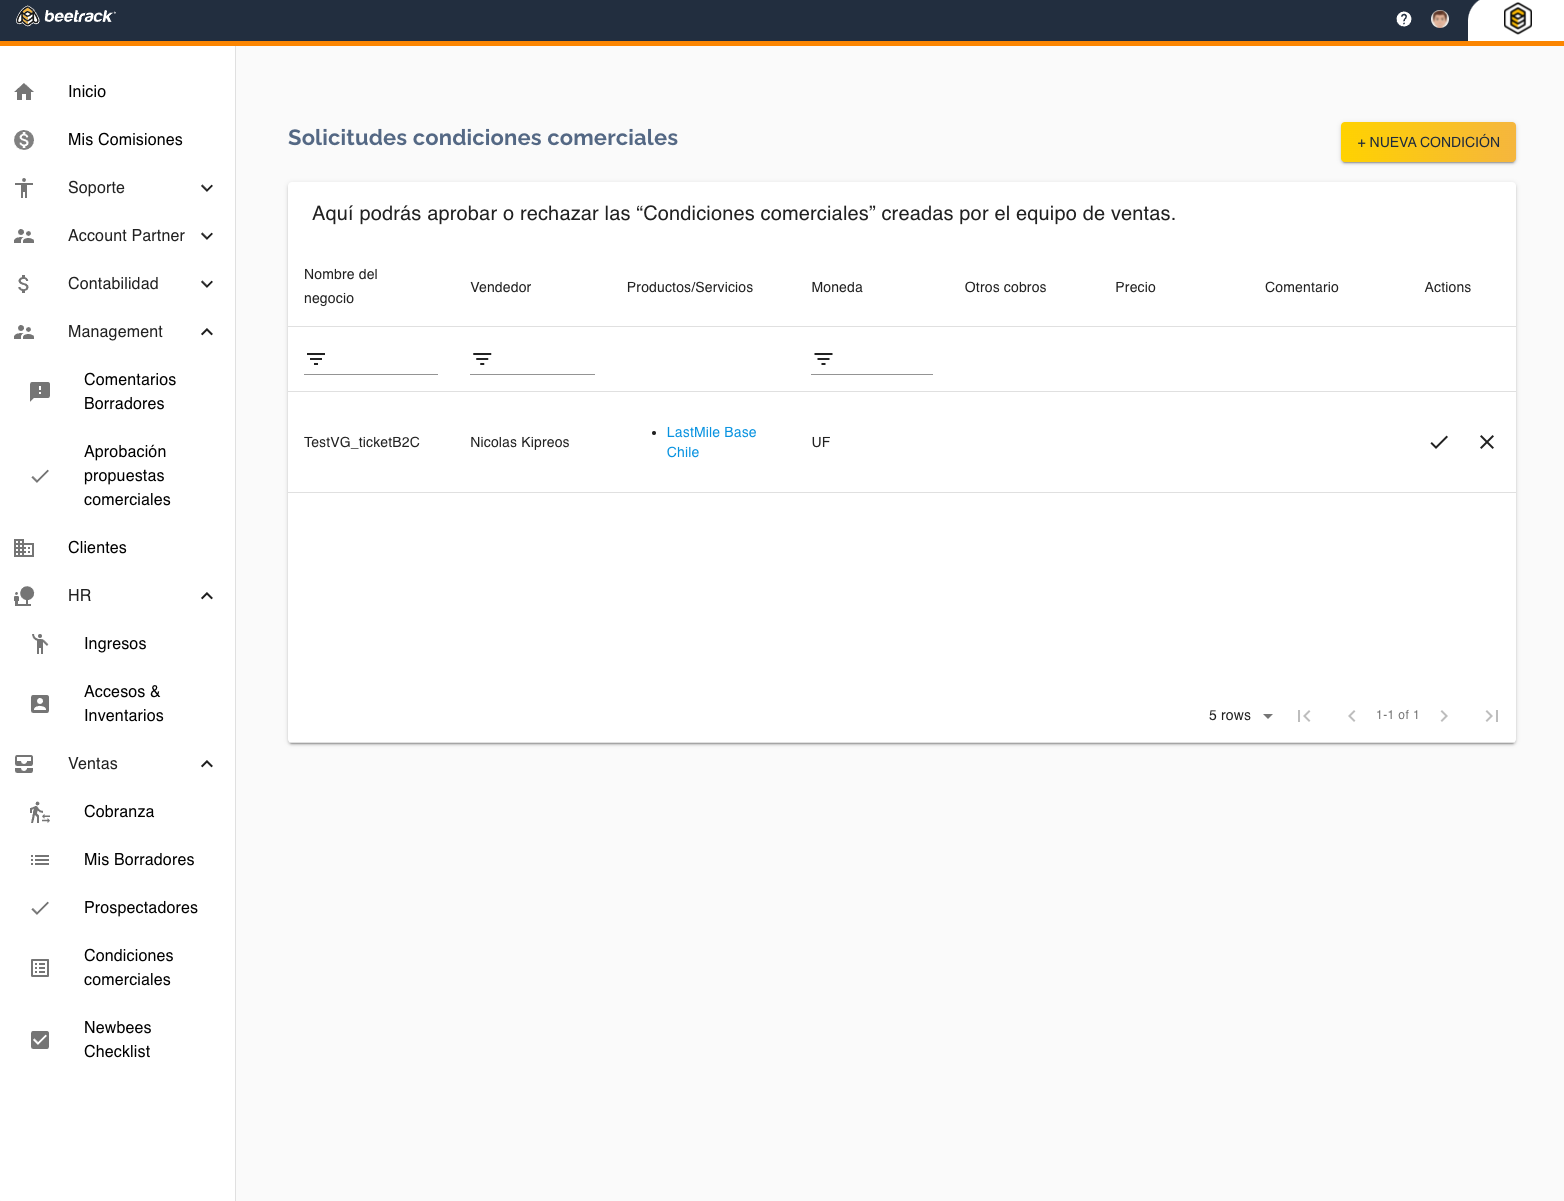
\includegraphics[width=0.6\linewidth]{figures/cc/vistas/cc_review.png}
      \caption{Vista de aprobación y rechazo de asociaciones comerciales.}
      \label{fig:cc_review}
    \end{figure}

    \begin{figure}
      \centering
      
\includegraphics[width=\linewidth]{figures/cc/mails/cc_approve_reject.jpeg}
      \caption{Correo electrónico de aprobación (izquierda) y rechazo (derecha) de asociación comercial.}
      \label{fig:cc_approve_reject}
    \end{figure}

    % vista de creacion de condicion comercial nueva desde cero por gerente

    En cuarto, y último lugar, se realizó un formulario totalmente personalizado para la creación de planes no estandarizados, tanto para productos como servicios. A este formulario no tienen acceso los vendedores, sino que solamente los gerentes. El propósito de esto es poder crear un plan totalmente a medida para un cliente en caso de que un plan estándar no permita abarcar el tipo de contrato que se cerró. Esta decisión de restricción del formulario a los gerentes se generó principalmente para evitar el fomentar que los vendedores vendan el producto de manera no estandarizada y que Beetrack se pueda acercar más a un SaaS tradicional. En la figura \ref{fig:cc_new_manager} se puede observar el formulario descrito anteriormente.
 
    \begin{figure}[H]
      \centering
      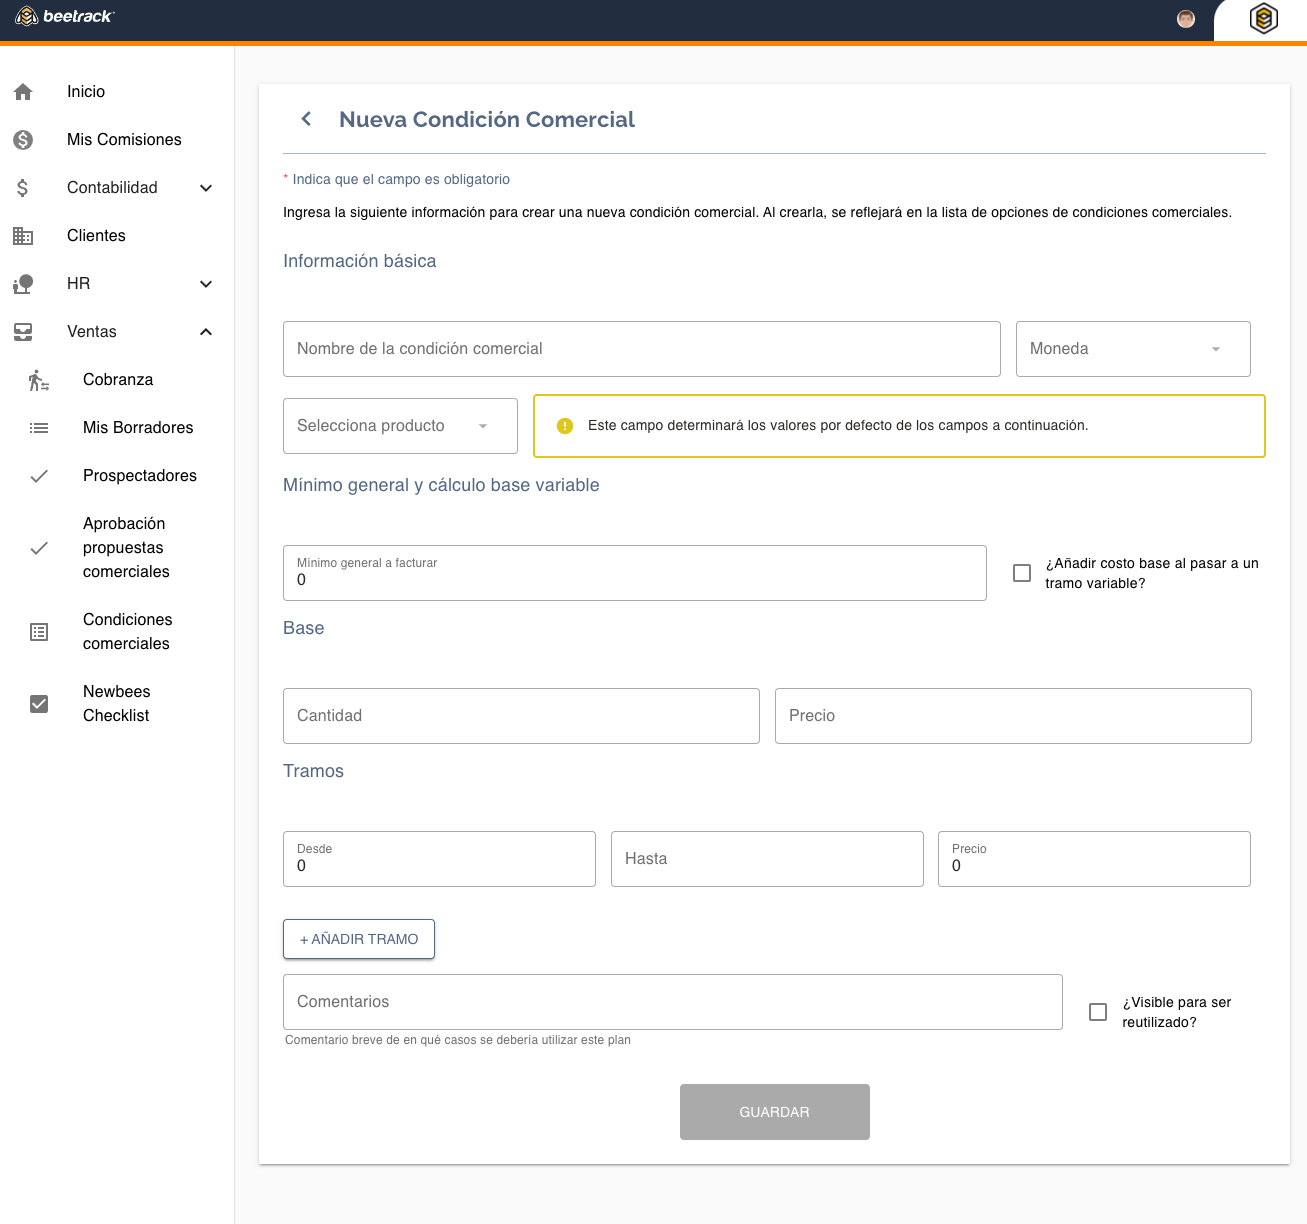
\includegraphics[width=0.6\linewidth]{figures/cc/vistas/cc_new_manager.png}
      \caption{Vista general de condiciones comerciales preaprobadas.}
      \label{fig:cc_new_manager}
    \end{figure}

\section{Resultados}

  Los resultados obtenidos para este proyecto estuvieron por sobre lo esperado en un comienzo. En particular se logró lo siguiente:

  \begin{enumerate}
    \item Servicio independiente de \textit{Hive}.
    
    Se creó un servicio independiente del ERP en RoR, que permitirá que se tenga la información descentralizada y se pueda enfocar en su única función de cálculo de costos y almacenamiento de planes de los clientes con tecnologías que no habían sido utilizadas dentro de la empresa anteriormente (GraphQL).

    \item Creación de modelos de planes flexibles.

    Se logró diseñar modelos de planes y condiciones lo suficientemente flexibles de manera que incluyeran todos los casos existentes y por existir. Junto a esto, la forma en que se abarcó el campo ``\texttt{condition}'' del modelo perimitió tener un \textit{solver} flexible que se adaptase a la forma de resolver el costo de los planes de manera correcta. Esta flexibilidad se logró mediante el trabajo entre múltiples áreas de la empresa, de manera de que se pudiese entender de mejor manera el problema existente. Al mismo tiempo, el esquema del modelo se logró definir gracias a un \textbf{análisis sistemático de los problemas} de los usuarios y trabajo en conjunto.

    \item Servicio con 87,9\% de precisión de facturación.
    
    Se creó un servicio de resolución de condiciones comerciales independiente del estado de los clientes, que permite calcular el costo asociado al uso de cada cliente, por producto, por servicio y por moneda. Esto permitió que se tenga una facturación mucho más exacta que otros intentos para la resolución de este problema, subiendo en más de un 40\% la precisión de la facturación de más de 700 facturas desde el último intento que fue en Hubspot con una certeza de 43\%. Esto se pudo lograr mediante una batería de \textbf{simulaciones de soluciones} y aplicación de \textbf{conocimientos avanzados de ingeniería de software} de manera de crear un \textit{software} escalable mediante diferentes patrones de diseño.

    \item Formularios de creación de condiciones.

    El alumo programó las vistas de \textit{frontend} dentro de \textit{Hive} mediante el diseño en conjunto con \textit{design ops}, resultando en los formularios especializados para los vendedores y el totalmente personalizable para los gerentes. Estos formularios quedaron \textbf{expresados en JavaScript} en el \textit{framework} de React.
    
    \item Vista de aprobación.
    
    Se desarrolló una vista especializada que permite que los gerentes de la empresa aprueben o rechacen las propuestas de asociaciones comerciales creadas por los vendedores en caso de que no sean tengan valores preaprobados. El objetivo de esta vista es poder tener una visión rápida de lo que están haciendo estos funcionarios de la empresa y también poder tener un control fino de qué tipos de condiciones comerciales se tiene para los clientes. Esta vista quedó plasmada en el lenguaje JavaScript en el \textit{framework} React.
    
    \item Correos de estado propuestas comerciales.
    
    Se crearon 3 correos automáticos que se envían en diferentes momentos acorde a los cambios de estado que ocurran para los planes y para las propuestas de asociaciones comerciales.

  \end{enumerate}